\documentclass[aspectratio=169]{xmu-slide}
% 如需 4:3 或 16:10 的比例,可将上面的 169 改为 43 或 1610

%%%%%%%%%%%%%%%%%%%%%%%%%%%%%%%%%%%%%%%%%%%%%%%%%%%%%%%%%%
%%%%%%%% XMU Undergraduates Thesis Slide Template %%%%%%%%
%%%%%%%%             Made by: F5Soft              %%%%%%%%
%%%%%%%%  https://github.com/F5Soft/xmu-template  %%%%%%%%
%%%%%%%%%%%%%%%%%%%%%%%%%%%%%%%%%%%%%%%%%%%%%%%%%%%%%%%%%%

% 取消注释可自定义颜色
% 深蓝色示例
% \definecolor{xmublue}{RGB}{0,68,170}
% \definecolor{xmulightblue}{RGB}{200,222,255}
% 橙色示例
% \definecolor{xmublue}{RGB}{249,138,0}
% \definecolor{xmulightblue}{RGB}{255,231,200}
% 粉色示例
% \definecolor{xmublue}{RGB}{219,115,188}
% \definecolor{xmulightblue}{RGB}{255,206,239}

% 取消注释可自定义字体(例如使用 macOS 下更好看的字体)
% \setsansfont{SF Pro}
% \setCJKsansfont{PingFang SC}

% 浅色主题 / 深色主题(注释即为浅色)
\dark

% 底部控制放映的导航条(取消注释则不显示)
\nav

% 封面的毕设题目
\title{厦门大学本科毕业论文幻灯片LaTeX模版}

% 答辩人
\author{你的名字}

% 指导教师
\teacher{你的导师\;职称}

% 答辩时间
\pubdate{2022-05-15}

\begin{document}

% 封面
\maketitle

% 目录页
\begin{frame}{目录}
    \tableofcontents
\end{frame}

% 第一部分 转场
\xmusection{第一部分的标题}{第一部分的简要说明,或标题的英文翻译}

\begin{frame}{当前帧的顶部标题}
    \color{red}本幻灯片模版完全由F5Soft自行编写。\color{black}同仓库下对应的论文模版则基于厦门大学图书馆i学堂LaTeX讲座中提供的硕博毕业论文模版改编而来。\par
    本模版支持列表、文本框、公式、插图、表格等元素,支持4:3,16:9,16:10等多种比例,并可自动生成目录、封面和章节转场页面。\par
    \color{red}对于复杂的图形绘制需求,建议使用draw.io、visio等工具绘制好后,导出成PDF格式,并通过figure环境直接插入幻灯片中。
\end{frame}

\begin{frame}{列表的例子}
    \begin{itemize}
        \item Point A
        \item Point B
        \pause
        \item 可通过pause命令让列表部分显示,而页码不变
              \begin{itemize}
                  \item part 1
                  \item part 2
              \end{itemize}
        \pause
        \item 用LaTeX制作幻灯片所用到的命令和用LaTeX写作时类似,例如数学环境同样使用\$符号包围: \par
              $x^2+y^2=z^2$、$\sqrt[3]{2}-\ln x=\mu$
    \end{itemize}
\end{frame}

\begin{frame}{列表的例子2}
    \begin{description}
        \item[API] Application Programming Interface
        \item[LAN] Local Area Network
        \item[ASCII] American Standard Code for Information Interchange
    \end{description}
    \begin{enumerate}[I]
        \item Point A
        \item Point B
              \begin{enumerate}[i]
                  \item part 1
                  \item part 2
              \end{enumerate}
    \end{enumerate}
\end{frame}

\begin{frame}{两栏的例子}
    \begin{columns}
        \column{0.5\textwidth}
        \qquad 主修专业毕业论文(设计)封面使用 160g 白色双胶纸,辅修封面为 160g 浅黄色皮纹纸。内页均为 A4 规格 80g 双胶纸。\par
        章的标题占2行,标题以外的文字为1.5倍行距。\par
        \qquad 换行时,如果要保留首行缩进,可使用qquad命令产生两个全角空白\par
        \column{0.5\textwidth}
        \begin{figure}
            
\includegraphics[width=0.8\textwidth]{xmu-logo-text.jpg}
            \caption{同样可以使用figure环境添加插图和字幕}
        \end{figure}
    \end{columns}
\end{frame}

\xmusection{第二部分的标题}{Title of Part 2}

\begin{frame}[plain]
    可使用plain选项添加完全空白的帧。\par
    如果创建帧的时候省略标题,则上方的标题和校徽均不会显示。
\end{frame}

\begin{frame}{用于强调内容的文本框示例}
    \begin{block}{泰勒展开}
        对于$\forall x\geq 0$,有
        $$
            e^x \leq x+\frac{x^2}{2}+\frac{x^3}{6}+\frac{x^4}{24}
        $$
        成立
    \end{block}
    \begin{block}{黎曼猜想的证明如下}
        Lorem ipsum dolor sit amet, consectetur adipisicing elit,
        sed do eiusmod tempor incididunt ut labore et
        dolore magna aliqua.
    \end{block}
\end{frame}

\begin{frame}{用于强调内容的文本框示例2}
    \begin{beamercolorbox}[center]{palette secondary}
        \vskip 0.5ex
        彩色盒子1\par
        可参考模版中封面部分的代码\par
        使用setbeamercolor命令设置自定义的盒子前景色和背景色
        \vskip 1em
    \end{beamercolorbox}
    \vskip 1em
    \begin{beamercolorbox}[center]{palette primary}
        \vskip 0.5ex
        彩色盒子2
        \vskip 1em
    \end{beamercolorbox}
\end{frame}

\begin{frame}{表格示例}
    \begin{table}
        \caption{基本资料表}
        \begin{tabular}{lllll}
            \toprule
            \bf 字段名称 & \bf 字段类型 & \bf 长度 & \bf 字段描述 & \bf 备注 \\ \midrule
            账户号      & Number   & 30     &          & 主键     \\
            密码       & Number   & 30     & 加密       &        \\
            姓名       & Varchar  & 50     &          &        \\
            电子邮箱     & Varchar  & 50     & VIP客户必填  &        \\ \bottomrule
        \end{tabular}
    \end{table}
\end{frame}

\begin{frame}{绘图示例}
    \begin{figure}
        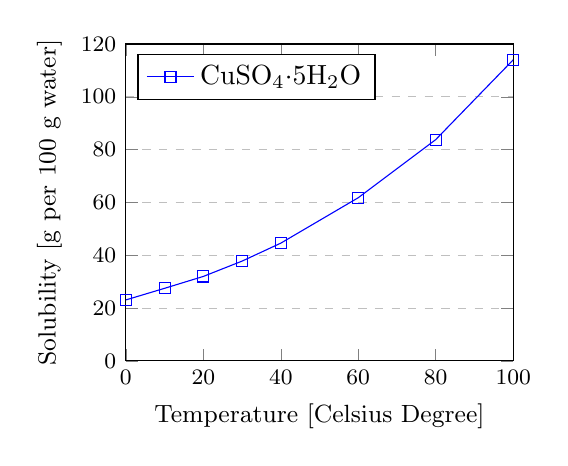
\begin{tikzpicture}
            \begin{axis}[
                    small,
                    xlabel={Temperature [Celsius Degree]},
                    ylabel={Solubility [g per 100 g water]},
                    xmin=0, xmax=100,
                    ymin=0, ymax=120,
                    xtick={0,20,40,60,80,100},
                    ytick={0,20,40,60,80,100,120},
                    legend pos=north west,
                    ymajorgrids=true,
                    grid style=dashed,
                ]
                \addplot[
                    color=blue,
                    mark=square,
                ]
                coordinates {
                        (0,23.1)(10,27.5)(20,32)(30,37.8)(40,44.6)(60,61.8)(80,83.8)(100,114)
                    };
                \legend{CuSO\(_4\cdot\)5H\(_2\)O}
            \end{axis}
        \end{tikzpicture}
        \caption{Temperature dependence of CuSO\(_4\cdot\)5H\(_2\)O solubility}\label{plot}
    \end{figure}
\end{frame}

% 谢谢收听页面
\thanksforlistening{请各位老师批评指正}

\end{document}